% !Mode:: "TeX:UTF-8"
\chapter{基于树形条件随机场的快速精准成分句法分析}
\label{cha:con-crf}

\section{引言}
\input{figures/tree.tex}
给定一个句子,成分句法分析旨在构建一个层次化的树结构. 如图\ref{fig:const-tree-full-figure},其中每个叶子结点是输入句子的每个词,而非终端结点作为组块(Constituents),如\texttt{$VP_{3,5}$}.

As a fundamental yet challenging task in the natural language processing (NLP) field, constituency parsing has attracted a lot of research attention since large-scale treebanks were annotated,  such as Penn Treebank (PTB), Penn Chinese Treebank (CTB), etc.
Parsing outputs are also proven to be extensively useful for a wide range of downstream applications \cite{akoury-etal-2019-syntactically,wang-etal-2018-tree}.
% 暂时不加参考文献了,太多了。
% like sematic parsing \cite{jiang-etal-2019-hlt,li-etal-2017-modeling,}, relation extraction \cite{qian-etal-2008-exploiting}, and machine translation .

As one of the most influential works, \cite{collins-1997-three} extends methods from probabilistic context-free grammars (PCFGs) to lexicalized grammars.
Since then, constituency parsing has been dominated by such generative models for a long time, among which
the widely used Berkeley parser adopts an unlexicalized PCFG with latent non-terminal splitting annotations \cite{matsuzaki-etal-2005-probabilistic,petrov-klein-2007-improved}.
As for discriminative models, there exist two representative lines of research.
The first line adopts the graph-based view based on dynamic programming decoding, using either local max-entropy estimation \cite{kaplan-etal-2004-speed} or global max-margin training \cite{taskar-etal-2004-max}.
The second group builds a tree via a sequence of shift-reduce actions based on greedy or beam decoding, known as the transition-based view \cite{sagae-lavie-2005-classifier,zhu-etal-2013-fast}.


\input{figures/tree.tex}

Recently, constituency parsing has achieved significant progress thanks to the impressive capability of deep neural networks in context representation.
Two typical and popular works are respectively the transition-based parser of \cite{cross-huang-2016-span} and the graph-based parser of \cite{stern-etal-2017-minimal}.
As discriminative models, the two parsers share several commonalities, both using 1) multi-layer BiLSTM as encoder; 2) minus features from BiLSTM outputs as span representations; 3) MLP for span scoring; 4) max-margin training loss.
Most works \cite{gaddy-etal-2018-whats,kitaev-klein-2018-constituency} mainly follow the two parsers and achieve much higher parsing accuracy than traditional non-neural models, especially with contextualized word representations trained with language modeling loss on large-scale unlabeled data \cite{peters-etal-2018-deep,devlin-etal-2019-bert}.

Despite the rapid progress, existing constituency parsing research suffers from two closely related drawbacks. First, parsing (also for training) speed is slow and can hardly satisfy the requirement of %for online parsing in
real-life systems.
Second, the lack of explicitly modeling tree/subtree probabilities may hinder the effectiveness of utilizing parsing outputs.
On the one hand, estimating probability distribution is one of the core issues in the NLP field \cite{le-zuidema-2014-inside}. On the other hand, compared with unbounded tree scores, tree probabilities can better serve high-level tasks as soft features \cite{jin-etal-2020-relation},
%are intuitively more useful than unbounded tree scores
and marginal probabilities of subtrees can support
the more sophisticated Minimum Bayes Risk (MBR) decoding \cite{smith-smith-2007-probabilistic}.

In fact, \cite{finkel-etal-2008-efficient} and \cite{durrett-klein-2015-neural} both propose CRF-based constituency parsing by directly modeling the conditional probability. % $p(\boldsymbol{t}\mid\boldsymbol{x})$.
However, both models are extremely inefficient due to
the high time-complexity of the inside-outside algorithm for loss and gradient computation, especially the outside procedure.
The issue becomes more severe in the DL era since all previous works perform the inside-outside computation on CPUs according to our knowledge and switching between GPU and CPU is expensive.
%unmatched speed of CPU/GPU computations.

%lafferty也得引用! 2001

This work proposes a fast and accurate CRF constituency parser by substantially extending the graph-based parser of \cite{stern-etal-2017-minimal}. The key contribution is that we batchify the inside algorithm for direct loss and gradient computation on GPU. Meanwhile, we find that the outside algorithm can be efficiently fulfilled by automatic back-propagation, which is shown to be equally efficient with the inside (forward) procedure, naturally verifying the great theoretical work of \cite{eisner-2016-inside}.
Similarly, we batchify the Cocke–Kasami–Younger (CKY) algorithm for fast decoding.

In summary, we make the following contributions.
% \footnote{Our code is available at \url{https://github.com/yzhangcs/crfpar}}
\begin{itemize}
    \item We for the first time propose a fast and accurate CRF constituency parser for directly modeling (marginal) probabilities of trees and subtrees.
          The efficiency issue, which bothers the community for a long time, is well solved by elegantly batchifying the inside and CKY algorithms for direct computation on GPU.
          % CRF batchify fully utilize the GPU power, directly compute on GPU. We for the first time introduce CRF to deep neural networks for constituency parsing, outperforming the max-margin methods.
          % \footnote{To our knowledge, this is the first BiLSTM-based CRF parser for constituency parsing.}

          % We propose to batchify the inside method, which makes it possible for parallelized large tensor computation on GPU. We also show that the sophisticated outside algorithm is no longer necessary, and can be replaced by the equally efficient back-propagation process for the computation of gradients and marginal probabilities.

    \item We propose a two-stage bracketing-then-labeling parsing approach that is more efficient and achieves slightly better performance than the one-stage method.

          %We borrow the architecture from biaffine parser, and exploit their advantages in the constituency parsing. All of these contribute to the fast (over 1,000 sentences per second) and accurate parsing.

    \item We propose a new span scoring architecture based on span boundary representation and biaffine attention scoring, which performs better than the widely used minus-feature method. %scoring  better scoring architecture (biaffine) and better parameter settings such as dropouts. substantially improve performance.
          We also show that the parsing performance can be improved by a large margin via better parameter settings such as dropout configuration.

    \item Experiments on three English and Chinese benchmark datasets show that our proposed two-stage CRF parser achieves new state-of-the-art parsing performance under both settings of w/o and w/ BERT \cite{devlin-etal-2019-bert}).
          In terms of parsing speed, our parser can parse over 1,000 sentences per second.

          %     %In the closed scenario that does not use any external resources, all of them achieve the state-of-the-art parsing results. Release code and models at github.
          %     Speed: 1,000 sentences per second.
          % new state-of-the-art results under several settings on three benchmark datasets of English and Chinese.

\end{itemize}


\begin{figure}[tb]
    \centering
    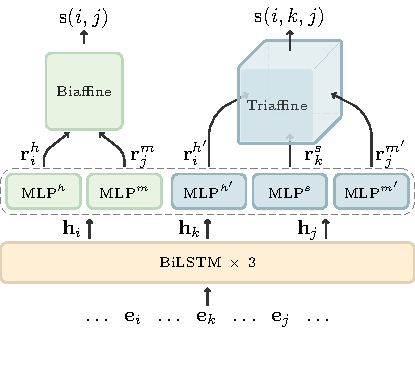
\includegraphics [scale=0.8] {figures/framework.pdf}
    \caption{Model architecture.
    }
    \label{fig:framework}
\end{figure}

\section{基线模型}

\subsection{模型定义}
本章所有方法都建立在目前性能最好的依存句法分析模型BiaffineParser\cite{dozat2017deep}的基础上.
作为基于图的句法分析模型,BiaffineParser采用双仿射运算计算有向完全图中每条弧的得分,最后通过MST算法(Minimum Spanning Tree),得到一棵最大生成树.

BiaffineParser采用如图\ref{fig:biaffineparser}所示的结构来计算弧$i \leftarrow j$的得分$\texttt{score}\left( i \leftarrow j \right)$,其中包含了BiLSTM编码层,MLP层(线性层)和Biaffine得分层.
%模型结构如图\ref{fig:conversion_models}的中间部分所示,它由三个网络层组成,分别是BiLSTM编码层,MLP层和Biaffine得分层.
首先,对于输入句子$w_1w_2\dots w_n$($n$为句子词数),BiaffineParser用多层BiLSTM来编码句子的信息.
最底层BiLSTM第k个位置的输入为词$w_k$的词向量$\mathbf{e}^{w_k}$及其词性向量$\mathbf{e}^{t_k}$的拼接向量,即输入特征$\mathbf{x}_k=\mathbf{e}^{w_k} \oplus \mathbf{e}^{t_k}$. %$\mathbf{x}_i=$.
最顶层BiLSTM第k个位置的输出$\mathbf{r}_k$为正向LSTM输出$\stackrel{\rightarrow}{\mathbf{h}_k}$和反向LSTM输出$\stackrel{\leftarrow}{\mathbf{h_k}}$的拼接,即$\mathbf{r}_k=\stackrel{\rightarrow}{\mathbf{h}_k} \oplus \stackrel{\leftarrow}{\mathbf{h}_k}$.

然后,以计算弧$i \leftarrow j$的得分为例,词$w_i$和$w_j$在最顶层BiLSTM的输出,即$\mathbf{r}_i$和$\mathbf{r}_j$,
需分别经过$\textup{MLP}^\textup{D}$和$\textup{MLP}^\textup{H}$来获得词$w_i$作为修饰词的表示$\mathbf{r}_i^\textup{D}$,
以及词$w_j$作为核心词的表示$\mathbf{r}_j^\textup{H}$:
\begin{equation}\label{eq:mlp}
    %	\setlength{\abovedisplayskip}{9pt}
    %	\setlength{\belowdisplayskip}{9pt}
    \begin{split}
        \mathbf{r}_{i}^{\textup{D}} &= \textup{MLP}^\textup{D} \left(\mathbf{r}_i \right) \\
        \mathbf{r}_{j}^{\textup{H}} &= \textup{MLP}^\textup{H} \left(\mathbf{r}_j \right) \\
        %\mathbf{r}_{k}^{\textup D} &= {\textup{MLP}}^{\textup D} \left(\mathbf{h}_k^{seq} \right)
    \end{split}
\end{equation}

% \begin{equation}
% 	\label{eq:ner-evaluate}
% 	\setlength{\abovedisplayskip}{9pt}
% 	\setlength{\belowdisplayskip}{9pt}
% 	\begin{split}
% 	%Precision & = \frac{Correctly~~Tagged~~Entities}{Tagged~~Entities} \\
% 	%Recall & = \frac{Correctly~~Tagged~~Entities}{Total~~Entities} \\
% 	%F1 & = \frac{2 * Precision * Recall}{Precision + Recall} \\
% 	Precision & = \frac{TP}{TP + FP} \\
% 	Recall & = \frac{TP}{TP + FN} \\
% 	F1 & = \frac{2 * Precision * Recall}{Precision + Recall} \\
% 	\end{split}
% \end{equation}

% \begin{equation}
% 	\label{eq:math}
% 	\setlength{\abovedisplayskip}{9pt}
% 	\setlength{\belowdisplayskip}{9pt}
% 	\mathbf{y}^{\text{ner}}=\mathop{\arg\max}_{\mathbf{y} \in \mathbf{Y}_{\mathbf{x}}} P(\mathbf{x},\mathbf{y}\,|\,\mathbf{\theta})
% \end{equation}

最后采用双仿射(Biaffine)运算,计算出弧$i \leftarrow j$的得分$\texttt{score}(i \leftarrow j)$:
\begin{equation} \label{eq:biaffine}
    %score(i, j) =  \big[{{\mathbf r_i^{D}} \oplus {\mathbf{1}}} \big]^\textup T   W^b  \mathbf r_j^{H}
    \texttt{score}(i \leftarrow j) =  \left[
        \begin{array}{c}
            \mathbf{r}_{i}^{\textup D} \\
            1
        \end{array}
        \right]^\mathrm{T}
    \mathbf{W}^b  \mathbf{r}_{j}^{\textup H}
\end{equation}

训练时,原始的BiaffineParser采用局部的softmax损失函数作为优化目标.
由于目标端句法数据为局部标注数据,为了得到更好的句法模型性能,受Li等(2016)\cite{zhenghua-p16}启发,我们采用基于Tree-CRF的全局损失函数\cite{ma-xuezhe-i17-non-proj-crf}来训练句法模型.

\begin{figure}[hb!]
    %\vspace{-0.5em}
    \centering
    \includegraphics[angle=0,width=0.5\textwidth]{img/biaffine-parser-crop.pdf}
    \caption{BiaffineParser计算$\texttt{score}(i \leftarrow j)$的过程. }
    \label{fig:biaffineparser}
    %\vspace{-1.5em}
\end{figure}

\subsection{基于多任务学习的树库融合模型}
为了充分挖掘相关任务的语料信息,多任务学习同时训练多个任务,让所有语料都能贡献到每一个任务上.
Guo等(2016)\cite{guo2016universal}第一次采用多任务学习框架利用异构数据提升句法模型性能,并且性能优于Li等(2012)\cite{li2012exploiting}的无监督的树库转化方法.

受Guo等(2016)\cite{guo2016universal}的启发,我们将BiaffineParser句法分析模型扩展成多任务学习模型来融合源端树库和目标端树库,并作为有监督树库转化的基线模型.
如图\ref{fig:mlt}所示,源端句法模型和目标端句法模型作为两个任务同时训练,共享词/词性向量表和多层BiLSTM层参数,独立MLP层和Biaffine层参数.
其中,共享参数将学习源端规范和目标端规范的共同句法信息,独立参数将学习不同规范的独特之处.
但是,多任务学习天然具有一个缺点:任务间的相互增益仅仅建立在底层共享的参数上,没能充分利用各个任务的数据信息.

\begin{figure}[hb!]
    %\vspace{-0.5em}
    \centering
    \includegraphics[angle=0,width=0.5\textwidth]{img/mlt-crop.pdf}
    \caption{基于BiaffineParser的多任务学习模型. }
    \label{fig:mlt}
    %\vspace{-1.5em}
\end{figure}
此外,为了让转化模型能充分利用源端树库的信息,我们将多任务学习训练好的编码层参数(词/词性向量表和多层BiLSTM层参数)作为预训练参数,
加载到转化模型的编码层,并且不进行微调.

\section{有监督的树库转化方法}
%$d^{\texttt{src}}$
树库转化任务旨在将图\ref{fig:example-su-vs-hit-cdt}下方的源端树,转化为上方的目标端树.
因此,树库转化的关键在于如何充分利用源端树的信息来指导目标端树的生成.
具体而言,在BiaffineParser句法分析器的基础上,树库转化就是要利用源端树作为指导信息,更好地给任意目标端弧$i \leftarrow j$打分.

我们采用两种不同的方法来编码源端树的信息, 并将其融入到基于图的BiaffineParser句法分析模型中,实现了两种树库转化模型.
一种是通过自定义的模式来刻画源端树和目标端树的对应关系,并将模式映射为嵌入向量,称为基于模式嵌入(The Pattern Embedding)的树库转化方法;
一种是采用TreeLSTM来编码源端树中对应的最短路径,称为基于SP-TreeLSTM(The Shortest Path TreeLSTM)的树库转化方法.
\begin{figure}[tb!]

    \centering
    \includegraphics[angle=0,width=0.9\textwidth]{img/img_pat_treelstm-crop.pdf}
    \caption{两种转化模型计算$\texttt{score}(i \leftarrow j)$的过程. }
    \label{fig:conversion_models}
\end{figure}

%$parser^{\texttt{src}}$
\subsection{基于模式嵌入的树库转化方法}
基于模式的树库转化方法主要是受Li等(2012)\cite{li2012exploiting}工作的启发. 首先,他们使用源端树库训练一个源端句法模型;
然后利用该源端句法模型去解析目标端树库,从而构建了一份伪双树对齐数据;
最后他们从伪双树对齐数据的源端树中抽取了基于模式的特征,作为目标端句法模型的额外指导特征,从而训练了一个准确率更高的目标端句法模型.

然而,Li等(2012)\cite{li2012exploiting}采用的是基于传统离散特征的句法模型,并且模式特征的定义仅仅考虑了句法的结构关系,没有考虑到源端树的依存关系.
我们在神经网络的BiaffineParser句法分析器的基础上,实现了Li等(2012)\cite{li2012exploiting}基于模式的思想. 此外,为了充分利用源端树的信息,我们进行了一些有用的扩展.

\begin{table*}[hb]
    \centering
    \caption{模式对照表. }
    \label{tb:pattern_table}
    \begin{tabular}{c|cc}
        \hline
        目标端弧                          & 源端树中$w_i$和$w_j$的位置关系                                                                     & 模式                        \\
        \hline
        \multirow{7}{*}{$i \leftarrow j$} & $i \leftarrow j$                                                                                   & 一致关系(consistent)      \\
                                          & $i \leftarrow k \leftarrow j$                                                                      & 祖孙关系(grand)           \\
                                          & $i \leftarrow k \rightarrow j$                                                                     & 兄弟关系(sibling)         \\
                                          & $i \rightarrow j$                                                                                  & 逆反关系(reverse)         \\
                                          & $i \rightarrow k \rightarrow j$                                                                    & 逆祖孙关系(reverse grand) \\
        %\cline{2-3}
                                          & $i \leftarrow k \rightarrow m \rightarrow j$, $i \leftarrow k \leftarrow m \leftarrow j$, $\cdots$ & 距离为3                     \\
                                          & 依次类推                                                                                           & 距离为4-5、6和$\geq 7$      \\
        \hline
    \end{tabular}
\end{table*}

以目标端弧$i \leftarrow j$为例,
一方面,我们根据源端树中词$w_i$到词$w_j$的距离扩展了模式的种类;
具体地, 我们将Li等(2012)\cite{li2012exploiting}的模式“else”按照距离进行扩展,增加了四种模式,分别是距离3,4-5,6,$\geq 7$. 最终,如表\ref{tb:pattern_table}所示,共定义了9种模式.
%举个例子,如图xx为例,词$w_i$和词$w_j$在源端树中修饰关系相反,为模式,为爷孙关系,模式为,关系为模式"3".

另一方面,除了编码源端树的结构特征,我们还引入了源端树的依存关系信息.
即利用词$w_i$与其核心词的依存关系标签$l_i$,以及词$w_j$与其核心词的依存关系标签$l_j$.
此外,受SP-Tree方法的启发,我们在源端树中找到词$w_i$到词$w_j$的最短路径,
进而确定二者的公共祖先结点词$w_a$,并利用公共祖先结点$a$与其核心词的依存关系标签$l_a$.
最终,我们利用了依存关系标签$l_i$、$l_j$和$l_a$.

接下来,如图\ref{fig:conversion_models}左半部分所示,以计算弧$i \leftarrow j$的得分为例,我们详细介绍如何将模式等特征融合到BiaffineParser句法分析器中.
%进而指导目标端树的生成,完成从源端树到目标端树的转化任务.
首先,我们从源端树中获取模式特征和三个依存关系标签:
1)根据词$w_i$和词$w_j$在源端树中的位置关系,参照表\ref{tb:pattern_table}列出的所有模式种类,确定模式类型$p_{i \leftarrow j}$.
%举个例子,如图xx为例,词$w_i$和词$w_j$在源端树中修饰关系相反,为模式,为爷孙关系,模式为,关系为模式"3".
2)获得词$w_i$与其核心词的依存关系标签$l_i$,词$w_j$与其核心词的依存关系标签$l_j$,二者最近公共祖先词$a$与其核心词的依存关系标签$l_a$.
举个例子,如图\ref{fig:example_pe_sp}所示,当要预测目标端弧“$\mbox{我}\rightarrow \mbox{上学}$”时,在源端树中,二者的位置关系是“$\mbox{我} \leftarrow \mbox{叫} \rightarrow \mbox{上学}$”. 这种位置关系属于表\ref{tb:pattern_table}中的“$i \leftarrow k \rightarrow j$”,即“sibling”. 此外,$l_i$、$l_j$和$l_a$分别为“VOB”、“DBL”和“HED”.
然后,为了将抽取出的源端树特征融入到BiaffineParser中,我们将这些输入特征映射成向量表示.
1)我们根据模式集合和源端依存关系标签集合分别建立特征嵌入向量查询表,记为$\mathbf{E}^{pat}$和$\mathbf{E}^{l}$.
2) 通过查询$E^{pat}$,我们将$p_{i \leftarrow j}$映射为向量$\mathbf{e}^{p_{i \leftarrow j}}$;
相似地,我们将$l_i$,$l_j$,$l_a$,通过查询$E^{l}$,我们得到向量$\mathbf{e}^{l_i}$,$\mathbf{e}^{l_j}$,$\mathbf{e}^{l_a}$.
3)我们将模式向量和依存关系向量拼接起来,作为对源端树$d^{\texttt{src}}$的编码向量$\mathbf{r}^{pat}_{i \leftarrow j}$,即:
\begin{equation}\label{eq:pattern}
    %	\setlength{\abovedisplayskip}{9pt}
    %	\setlength{\belowdisplayskip}{9pt}
    \mathbf{r}^{pat}_{i \leftarrow j} = \mathbf{e}^{p_{i \leftarrow j}} \oplus \mathbf{e}^{l_i} \oplus
    \mathbf{e}^{l_j} \oplus \mathbf{e}^{l_a}
\end{equation}
至此,表示向量$\mathbf{r}^{pat}_{i \leftarrow j}$中蕴含了源端树的结构信息和依存关系信息.

最后,我们在BiaffineParser的基础上融合源端树的表示$\mathbf{r}^{pat}_{i \leftarrow j}$到目标端句法模型中,指导目标端树的构建.
即,将向量$\mathbf{r}^{pat}_{i \leftarrow j}$分别与$r_i$和$r_j$拼接($r_i$和$r_j$分别是BiaffineParser中词$w_i$和词$w_j$的BiLSTM层输出),
分别作为$\textup{MLP}^\textup{D}$和$\textup{MLP}^\textup{H}$的输入:
\begin{equation}\label{eq:pattern}
    %	\setlength{\abovedisplayskip}{9pt}
    %	\setlength{\belowdisplayskip}{9pt}
    \begin{split}
        \mathbf{r}_{i,i \leftarrow j}^{\textup{D}} &={\textup{MLP}}^{\textup{D}} \big(\mathbf{r}_i \oplus \mathbf{r}^{pat}_{i  \leftarrow j} \big)  \\
        \mathbf{r}_{j,i\leftarrow j}^{\textup{H}} &= {\textup{MLP}}^{\textup{H}} \big(\mathbf{r}_j \oplus \mathbf{r}^{pat}_{i \leftarrow j} \big)
    \end{split}
\end{equation}
通过$\mathbf{r}_{i,i \leftarrow j}^{\textup{D}}$和$\mathbf{r}_{i,i \leftarrow j}^{\textup{H}}$,
我们将源端树的结构信息和依存关系信息融入到了BiaffineParser中.

计算弧$i \leftarrow j$得分时,我们仍然采用公式\ref{eq:biaffine}中的双仿射运算:
%不同的是$\textup{MLP}^\textup{H}$和$\textup{MLP}^\textup{D}$的输入多了源端树的编码信息$\mathbf{r}^{pat}_{i \leftarrow j}$
\begin{equation} \label{eq:biaffine_pat}
    %score(i, j) =  \big[{{\mathbf r_i^{D}} \oplus {\mathbf{1}}} \big]^\textup T   W^b  \mathbf r_j^{H}
    %	\setlength{\abovedisplayskip}{9pt}
    %	\setlength{\belowdisplayskip}{9pt}
    \texttt{score}(i \leftarrow j) =  \left[
        \begin{array}{c}
            \mathbf{r}_{i,i \leftarrow j}^{\textup{D}} \\
            1
        \end{array}
        \right]^\mathrm{T}
    \mathbf{W}^b  \mathbf{r}_{i,i \leftarrow j}^{\textup{H}}
\end{equation}
从上述的计算过程看,通过$\mathbf{r}_{i,i \leftarrow j}^{\textup{D}}$和$\mathbf{r}_{i,i \leftarrow j}^{\textup{H}}$,我们将源端树的信息贡献到弧$i \leftarrow j$的分数$\texttt{score}(i \leftarrow j)$计算中.

\begin{figure}[hb]
    %\vspace{-0.5em}
    \centering
    \includegraphics[angle=0,width=0.9\textwidth]{img/example-pe-sp-crop.pdf}
    \caption{预测弧$\mbox{我}\rightarrow \mbox{上学}$时,两种转化方法使用的源端树信息. }
    \label{fig:example_pe_sp}
    %\vspace{-1.5em}
\end{figure}

\subsection{基于SP-TreeLSTM的树库转化方法}
不同于基于模式嵌入的浅层编码方式,
%本节采用树状长短期记忆网络(TreeLSTM)从深层编码源端树的信息.
本节采用树状LSTM(TreeLSTM)深度编码源端树的信息.
TreeLSTM是由Tai等(2015)\cite{tai2015improved}通过扩展LSTM设计而成的用于编码树结构数据的神经网络层.
他们通过TreeLSTM来编码依存句法树,从而将句法信息融入到语义相关性任务和情感分析任务中.
Miwa和Bansal(2016)\cite{miwa-p16-treelstm-re}在关系抽取任务上比较了三种TreeLSTM的变种,其中编码最短路径树的SP-TreeLSTM方法取得了最好的性能.
%miwa等在关系抽取任务上比较了三种TreeLSTM的变种,
%即用于编码整棵句法树的Full-tree TreeLSTM, 编码最小子树的Sub-tree TreeLSTM,以及编码最短路径树的SP-TreeLSTM.
%其实验结果表明SP-TreeLSTM给模型性能带来了更大的提升.
%% 此外在树库转化任务上,采用SP-Tree LSTM编码源端树信息同样取得了更优的性能,与miwa等的结论一致.
%因此,我们采用SP-TreeLSTM来编码源端树信息,并融入到BiaffineParser中,完成源端树到目标端树的转化.

借鉴Miwa和Bansal(2016)\cite{miwa-p16-treelstm-re},我们也采用SP-TreeLSTM来编码源端树信息,并融入到BiaffineParser句法分析器中.
顾名思义,SP-TreeLSTM编码的不是一棵完整的树,而是只编码了由两个词确定的一棵最短路径树.
这里我们给出最短路径树的定义:当给定一棵树和两个节点$i$和$j$时,我们能找到唯一确定的最近公共祖先节点$a$,
那么最短路径树即为由从节点$i$到节点$a$,再从节点$a$到节点$j$的两条路径组成的一棵树(一般情况下由两条路径组成).
如图\ref{fig:example_pe_sp}所示,当要预测目标端弧“$\mbox{我}\rightarrow \mbox{上学}$”时,源端树中黑线标出的两条弧即为对应的最短路径树(灰色标出的弧不参与计算).

如图\ref{fig:conversion_models}的右半部分所示,我们采用双向SP-TreeLSTM编码最短路径树的信息(即自底向上和自顶向下两个方向).
自底向上的 SP-TreeLSTM 的信息流从叶子节点开始,沿着依存弧的反方向一直流向根节点(黑色虚线) ,
而自顶向下的 SP-TreeLSTM 的信息流从根节点开始,沿着依存弧的方向一直流到每一个叶子节点(蓝色虚线) .

为了让SP-TreeLSTM能充分利用句子的文本信息,
我们将SP-TreeLSTM层堆叠在BiaffineParser句法分析器的BiLSTM层的上方,即将顶层BiLSTM的输出作为TreeLSTM的输入.
此外,为了引入源端树的依存关系信息,我们将源端树的依存关系标签映射为嵌入向量,作为TreeLSTM的额外输入.
例如,TreeLSTM中$w_k$节点的输入为$x_k=
    \mathbf{r_k} \oplus \mathbf{e}^{l_k}$,
其中$\mathbf{r}_k$是顶层BiLSTM在词$w_k$处的输出向量,$l_k$是源端树中词$w_k$与其核心词的依存关系标签,$\mathbf{e}^{l_k}$是$l_k$的嵌入向量.

对于自底向上的TreeLSTM,任意一个节点的隐状态向量由该节点的输入向量$\mathbf{x}_k$和源端句法树中该节点所有孩子节点的隐状态向量经过计算得到.
公式\ref{eq:sp_treelstm}表明了获得词$w_k$的TreeLSTM隐状态向量$\mathbf{h}_k$的计算过程:
\begin{equation}\label{eq:sp_treelstm}
    %\begin{small}
    %	\setlength{\abovedisplayskip}{9pt}
    %	\setlength{\belowdisplayskip}{9pt}
    \begin{split}
        %x_{t} &= r^{seqLstm}_t \oplus e^{label}_t \\
        \Tilde{\mathbf{h}}_a &= \sum_{k \in \mathcal{C}(a)} \mathbf{h}_k \\
        \mathbf{i}_a &= \sigma \left( \mathbf{U}^{(i)} \mathbf{x}_a + \mathbf{V}^{(i)} \Tilde{\mathbf{h}}_a + \mathbf{b}^{(i)} \right) \\
        \mathbf{f}_{a,k} &= \sigma \left( \mathbf{U}^{(f)} \mathbf{x}_a +  \mathbf{V}^{(f)} \mathbf{h}_k + \mathbf{b}^{(f)} \right)   \\
        \mathbf{o}_{a} &= \sigma \left( \mathbf{U}^{(o)} \mathbf{x}_a + \mathbf{V}^{(o)} \Tilde{\mathbf{h}}_a + \mathbf{b}^{(o)} \right) \\
        \mathbf{u}_{a} &= \tanh \left( \mathbf{U}^{(u)} \mathbf{x}_a + \mathbf{V}^{(u)} \Tilde{\mathbf{h}}_a + \mathbf{b}^{(u)} \right) \\
        \mathbf{c}_{a} &= \mathbf{i}_a \odot \mathbf{u}_a + \sum_{k \in \mathcal{C}(a)} \mathbf{f}_{a,k} \odot \mathbf{c}_k \\
        \mathbf{h}_{a} &= \mathbf{o}_a \odot \tanh \big(\mathbf{c}_a\big) \\
    \end{split}
    %\end{small}
\end{equation}
其中$\mathcal{C}(a)$是最短路径树中节点$k$的所有孩子节点的集合,$\mathbf{f}_{a,k}$是节点$k$的孩子节点$m$的遗忘向量.

对于自顶向下 的SP-TreeLSTM,任意一个节点的由该节点的输入向量$\mathbf{x}_k$和
源端句法树中其父亲节点的隐状态向量经过计算得到.
计算过程和公式\ref{eq:sp_treelstm}一致,其中$\mathcal{C}(a)$是节点$k$的父亲节点的集合(只有一个父亲),
$\mathbf{f}_{a,k}$是节点$k$的父亲节点$m$的遗忘向量.

经过双向SP-TreeLSTM编码层之后,
我们得到了最短路径树中每个词的自底向上TreeLSTM的隐状态向量$\mathbf{h}^{\uparrow}$和自顶向下TreeLSTM的隐状态向量$\mathbf{h}^{\downarrow}$.
为了更好地表示最短路径树的信息,借鉴Miwa和Bansal(2016)\cite{miwa-p16-treelstm-re}的做法,我们将词$w_i$的自顶向下TreeLSTM的输出$\mathbf{h}_i^{\downarrow}$,
词$w_j$的自顶向下的输出$\mathbf{h}_j^{\downarrow}$,和词$w_a$的自底向的输出$\mathbf{h}_a^{\uparrow}$拼接起来作为源端树的编码向量:
\begin{equation}
    \label{eq:sp_treelstm_rep}
    %	\setlength{\abovedisplayskip}{9pt}
    %	\setlength{\belowdisplayskip}{9pt}
    \mathbf{r}^{tree}_{i \leftarrow j} = \mathbf{h}_i^{\downarrow} \oplus \mathbf{h}_j^{\downarrow} \oplus \mathbf{h}_a^{\uparrow}
\end{equation}
%如图xx所示,我们把每个词的$h^{\uparrow}$和$h^{\downarrow}$拼接,作为该词在双向SP-Tree LSTM的输出向量.
%例如词$w_i$的双向SP-Tree LSTM的输出向量$r_i^{tree}=$
然后,类似于公式\ref{eq:pattern},
我们将弧$i \leftarrow j$在源端树中的编码向量$\mathbf{r}^{tree}_{i \leftarrow j}$
作为$\textup{MLP}^{\textup{D}}$和$\textup{MLP}^{\textup{H}}$的额外输入,融入到BiaffineParser中:
\begin{equation}\label{eq:mlp_treelstm}
    %	\setlength{\abovedisplayskip}{9pt}
    %	\setlength{\belowdisplayskip}{9pt}
    \begin{split}
        \mathbf{r}_{i,i \leftarrow j}^{\textup{D}} &={\textup{MLP}}^{\textup{D}} \big(\mathbf{r}_i \oplus \mathbf{r}^{tree}_{i  \leftarrow j} \big)  \\
        \mathbf{r}_{j,i\leftarrow j}^{\textup{H}} &= {\textup{MLP}}^{\textup{H}} \big(\mathbf{r}_j \oplus \mathbf{r}^{tree}_{i \leftarrow j} \big)
    \end{split}
\end{equation}
至此,我们通过表示$\mathbf{r}_{i,i \leftarrow j}^{\textup{D}}$和$\mathbf{r}_{i,i \leftarrow j}^{\textup{H}}$将源端树信息融入到了BiaffineParser中.
最后,我们采用公式\ref{eq:biaffine_pat}所示的双仿射运算,得到弧$i \leftarrow j$在源端树指导下的分数.

\section{实验结果及分析}

\subsection{实验设置}
\textbf{实验数据.  }
本章涉及到多个数据,包括源端树库HIT,目标端树库CODT,双树对齐树库$CODT^{\texttt{HIT}}$,转化后源端HIT树库. 我们将利用这些数据设计对比实验,验证采用树库转化方式利用源端树库的有效性.
图\ref{fig:datasets}给出了这些数据间的关系(详细请参考图
\ref{fig:data_anot}和图\ref{fig:conversion_pipeline}):从源端树中采样约11K的数据,按照CODT规范重新标注,形成CODT目标端树库,再和源端数据对齐后,形成双树对齐数据;通过树库转化任务产生符合目标端规范的转化后源端树库.

\begin{figure}[hb!]
    %\vspace{-0.5em}
    \centering
    \includegraphics[angle=0,width=0.9\textwidth]{img/datasets-crop.png}
    \caption{多个实验数据及其相互关系. }
    \label{fig:datasets}
    %\vspace{-1.5em}
\end{figure}

对于人工标注的双树对齐数据,我们随机选择1K/2K句作为Dev/Test集,剩下的约8K句子作为Train集. 如表\ref{tb:HIT-split}所示, 我们统计了Train/Dev/Test集中含有的句子数、标注的词数、总词数. %以及源端标注和目标端标注的一致性.
(由于采用Tree-CRF损失函数,我们删除了Train/Dev/Test集中的非投影树. )

\begin{table}[hb!]
    \centering
    \caption{数据统计. }
    \label{tb:HIT-split}
    \begin{tabular}{cccc}
        %\hline
        \toprule
                  & 句子数 & 总词数  & 标注词数 \\
        \midrule
        Train     & 7,768  & 119,707 & 36,348   \\ %\hline
        Dev       & 998    & 14,863  & 4,839    \\ %\hline
        Test      & 1,995  & 29,975  & 96,79    \\
        \midrule
        HIT-train & 52,450 & 980,791 & 36,348   \\
        \bottomrule
    \end{tabular}
\end{table}

\textbf{评价指标.  } 我们采用标准的UAS(unlabeled attachment score,只考虑依存弧的正确性)和LAS(labeled attachment score,同时考虑依存弧和依存关系的正确性)来评价句法模型、多任务学习模型和转化模型的性能.

\textbf{参数设置.  } 对于BiaffineParser,我们遵循了Dozat和Manning(2017)\cite{dozat2017deep}等的部分参数设置:使用100维的GloVe预训练词向量,100维的词性嵌入向量. 由于训练数据规模较小,为了训练更好的模型,我们将BiLSTM编码层的层数减小到2,输出维度减小为300,MLP层的维度减小为200和100.

对于转化模型,模式的嵌入向量维度为50,依存关系标签的维度为50(如公式\ref{eq:pattern},所以$\mathbf{r}^{pat}_{i \leftarrow j}$维度为200),SP-TreeLSTM的输出维度为100(如公式\ref{eq:sp_treelstm_rep},所以$\mathbf{r}^{tree}_{i \leftarrow j}$维度为300),MLP层维度为300和100.

训练阶段,我们的批处理大小为200个句子,训练完所有训练语料作为一次迭代,每迭代一次都会在Dev集上评估一次模型,当Dev集上的性能达到最优之后50次迭代性能未增长,则停止训练. 最后我们保存Dev集上性能最好的模型,并在Test集上进行评价.

对于多任务模型而言,为了平衡语料间规模的差异,我们按照训练100个HIT数据,再训练100个CODT数据的次序进行,以训练完一次CODT数据为一次迭代.

为了让转化模型能充分利用HIT-train中未被重新标注的句法树,我们将多任务学习训练好的编码层参数(词/词性向量表和多层BiLSTM层参数)作为预训练参数,加载到转化模型的编码层,并且不进行微调.


\subsection{树库转化的实验结果}
表\ref{tb:HIT-conversion-rst}给出了转化模型在Test集上的性能. 第2行给出了多任务学习方式训练的目标端句法模型在Test集上的性能.
与直接编码源端树的树库转化方法相比,该方法通过共享的编码层来间接利用源端树信息,我们将其作为树库转化方法的强基线模型.

第3、4行分别给出了基于模式嵌入的树库转化方法和基于SP-TreeLSTM的树库转化方法的性能,从UAS/LAS两个性能指标上看,两种方法取得了几乎相同的性能. 这与我们实验前的直觉不同,从两种转化方法对源端树的编码方法上看,基于TreeLSTM的深度编码方式理应优于基于模式的浅层编码方式.
与间接的多任务学习模型相比,树库转化模型进一步提升了目标端句法模型的性能,LAS上最多提升了7.58\%(82.09-74.51).

我们很自然地想到将两种转化方法结合起来,即将$\mathbf{r}^{tree}_{i \leftarrow j}$和$\mathbf{r}^{pat}_{i \leftarrow j}$拼接起来作为$\texttt{MLP}^{\texttt{D|H}}$层的输入. 第5行给出了结合两种树库转化方法的实验结果. 可以看出,两种方法结合到一起并没有进一步提升转化模型的性能,反而略有下降. 我们认为可能的原因是:两种方法虽然尝试从不同的角度去编码源端句法树信息,但是最终得到的句法信息是冗余的,而不是互补的.
\begin{table}[hb!]
    %\setlength{\leftskip}{-25pt}
    \centering
    %\begin{small}
    %\begin{tabular}{c |c| *{2}{c}}%  | *{2}{c} }
    \caption{Test集上的转化模型性能}
    \label{tb:HIT-conversion-rst}
    \begin{tabular}{c c c c}%  | *{2}{c} }
        \toprule
        %\multirow{2}{*}{}
        %& \multicolumn{2}{|c}{on Dev }
        %& \multicolumn{2}{|c}{on Test } \\
        %\cline{2-5}
                                                 & 训练数据                    & UAS            & LAS            \\ %& UAS & LAS \\
        \midrule
        %Single parsing & 75.42 & 70.21 \\ T
        多任务学习模型                           & \texttt{Train \& HIT-train} & 79.29          & 74.51          \\
        \midrule
        基于模式嵌入的树库转化模型(PatEmb)     & \texttt{Train}              & 86.66          & 82.03          \\
        基于SP-TreeLSTM的树库转化模型(SP-Tree) & \texttt{Train}              & \textbf{86.69} & \textbf{82.09} \\
        %Combined
        结合的方法(PatEmb+SP-Tree)             & \texttt{Train}              & 86.66          & 81.82          \\
        \bottomrule
    \end{tabular}
\end{table}

%{\bfseries{源端句法特征消融实验}}
\textbf{源端句法特征消融实验.  }
由于最终融合的句法信息由多个句法特征组成,如公式\ref{eq:pattern}所示,模式编码的句法信息由三个词的依存关系标签、模式等特征组成. 为了能更好地了解各个源端句法特征对转化模型的作用,我们做了特征消融实验. 如表\ref{tb:feature-ablation-conversion}所示,每个实验,我们从一个完整的转化模型中去掉一个源端句法特征.

对基于模式嵌入的转化方法而言,去除了对模式的扩展之后,所有的消融实验性能都有一定的下降,这表明了我们的扩展是有效的.
最有效的扩展是引入了源端树依存关系信息,其中最重要的依存关系特征是词$w_i$与其核心词的依存关系标签$l_i$,去除$l_i$后,LAS下降值最高,为0.88\%(82.03−81.15).
三个依存关系标签都去掉后,UAS上性能下降了0.73\%(86.66−85.93),LAS上性能降低了1.95\%(82.03−80.08),说明源端依存关系标签与目标端依存关系标签高度相关,对改善LAS有很大帮助.

对于基于SP-TreeLSTM的转化方法而言,源端依存关系标签的引入也非常有助于转化模型性能的提升. 加入源端依存关系标签后,在Test集上,UAS上性能提升了0.49\%(86.69−86.20),LAS上性能提升了 1.53\%(82.09−80.56).
\begin{table}[hb!]
    %\setlength{\leftskip}{-25pt}
    \centering
    \caption{转化模型的特征消融实验. }
    \label{tb:feature-ablation-conversion}

    %		\begin{tabular}{c | *{2}{c}  | *{2}{c} }
    \begin{tabular}{c  cc  cc}
        \toprule
        \multirow{2}{*}{}
                                                 & \multicolumn{2}{c}{ \texttt{Dev}  }
                                                 & \multicolumn{2}{c}{ \texttt{Test} }                                                    \\
        \cline{2-5}
                                                 & UAS                                 & LAS            & UAS            & LAS            \\
        \midrule
        基于模式嵌入的树库转化模型(PatEmb)     & \textbf{86.73}                      & \textbf{81.93} & \textbf{86.66} & \textbf{82.03} \\
        %\hline
        PatEmb - 路径距离扩展                    & 86.73                               & 81.75          & 86.57          & 81.94          \\
        %\hline
        PatEmb -  $l_i$                          & 86.47                               & 80.55          & 86.47          & 81.15          \\
        PatEmb - $l_j$                           & 86.55                               & 81.69          & 86.45          & 81.76          \\
        PatEmb - $l_a$                           & {86.24}                             & 81.66          & {86.17}        & 81.51          \\
        %\hline
        PatEmb - 所有依存关系标签                & 86.05                               & 79.78          & 85.93          & 80.08          \\
        %\hline
        \midrule
        基于SP-TreeLSTM的树库转化模型(SP-Tree) & \textbf{86.73}                      & \textbf{81.95} & \textbf{86.69} & \textbf{82.09} \\
        SP-Tree - 所有依存关系标签               & 86.55                               & 80.32          & 86.20          & 80.56          \\
        %w/o sep init state & 86.86 & 81.81	& 86.38 & 81.58 \\
        \bottomrule
    \end{tabular}

\end{table}


\subsection{利用转化后树库的实验结果}
虽然表\ref{tb:HIT-conversion-rst}中树库转化的性能要远远高于多任务学习方式训练的目标端句法模型的性能,但是树库转化模型无法直接用来解析纯文本,还需要源端句法树作为输入.
从改善目标端句法模型的角度看,用树库转化模型与多任务学习方式训练的目标端句法模型相比是不公平的.
所以从改善目标端句法模型性能的角度看,我们还需要回答以下两个问题:
1)源端树库的引入是否可以有效提升目标端句法模型的分析准确率?
2)进一步地,与多任务学习方式利用源端树库相比,通过树库转化方法得到的目标端句法模型能否带来更高的分析准确率?
%所以另一个需要回答的重要问题是,与多任务学习训练的目标端句法模型相比,通过树库转化方法得到的目标端句法模型能否带来更高的分析准确率.
%因此,我们利用树库转化方式扩大目标端树库规模并训练一个目标端句法模型,然后利用该目标端句法模型与多任务学习模型进行公平比较.
%我们利用训练好的树库转化模型,将HIT-train转化为符合目标端规范的数据. 然后将其与目标端树库合并到一起,训练一个目标端句法模型. 最后,我们利用该目标端句法模型与多任务学习模型进行对比.
%在句法模型简单性方面,树库转化方式得到的目标端句法模型更好,因为最终目标端句法模型直接在一个扩大的同构树库训练上,而不像多任务学习方法需要同时在两个异构树库上训练两个句法模型.

如图\ref{fig:parsers}所示,为了回答上述问题,我们训练了多个不同的句法模型构成一组对比实验,实验结果如表\ref{tb:final-results-with-converted data}所示. 值得注意的是,表中给出的实验结果看起来较低,主要原因是我们采用了局部标注的方式标注了最难识别的依存弧(意味着评价的弧也是最难的弧).
\begin{figure}[hb!]
    %\vspace{-0.5em}
    \centering
    \includegraphics[angle=0,width=0.9\textwidth]{img/parsers-crop.pdf}
    \caption{多个句法模型之间的对比. }
    \label{fig:parsers}
    %\vspace{-1.5em}
\end{figure}

%表\ref{tb:final-results-with-converted data}给出了采用不同方法利用源端数据训练的目标端句法模型的性能.


第2行给出了只利用人工标注的目标端数据训练的句法模型的性能,作为其他目标端句法模型的基线模型(如图\ref{fig:parsers}-(a)所示).

由于源端树库HIT和目标端树库CODT具有很高的一致性,我们尝试利用异构的源端树库HIT来训练源端句法模型(如图\ref{fig:parsers}-(b)所示),并利用目标端CODT的Test集来评估该模型的性能. 考虑到二者的依存关系标签集合不同,我们将源端HIT的依存关系标签映射成目标端CODT的标签标签后,再去评价LAS指标. 从第3行的实验结果看,利用源端树库训练的句法模型比基线模型能更好的预测出依存弧,UAS上提升了0.21\%(76.20−75.99). 我们认为可能的原因是:源端异构树库虽然存在一定的差异,但考虑到HIT和CODT的依存弧一致性高且HIT规模大,HIT包含了更多的目标端训练数据,因此取得了更好的UAS性能. 另一方面也表明了对于依存句法分析任务而言,数据规模是提升句法模型性能的一个关键因素. 从LAS上看,源端树库训练的句法模型要逊色于目标端句法模型,降低了2.52\%(70.95-68.43). 可能的原因是HIT和CODT依存关系的一致性不够高,存在了大量的噪音,干扰了模型的学习.

第4行给出了采用多任务学习方法来利用源端树库时(如图\ref{fig:parsers}-(c)所示),训练得到的目标端句法模型的性能. 相较于基线模型,多任务学习模型在UAS和LAS上分别提升了3.30\%和3.56\%(79.29-75.99,74.51-70.95),表明了多任务学习模型可以有效地利用源端树库HIT来帮助目标端句法模型,间接弥补了目标端训练数据规模小的问题.

第5行给出了利用转化后HIT数据训练的目标端句法模型性能(如图\ref{fig:parsers}-(d)所示). 具体而言,我们用基于SP-TreeLSTM训练的树库转化模型将源端树库HIT转化为符合目标端规范的树库,然后与小规模目标端树库CODT合并成为一份训练数据,并训练一个目标端句法模型. 可以看出,相较于基线模型,树库转化方法能有效的利用源端树库,UAS和LAS上分别提升了4.46\%,4.88\%(80.45-75.99,75.83-70.95). 相较于多任务学习模型,树库转化方式对源端树库的使用更加充分,UAS和LAS上分别进一步提高了1.16\%,1.32\%(80.45-79.29,75.83-74.41).

\begin{table}[hb!]
    %\setlength{\leftskip}{-25pt}
    \centering
    \caption{不同句法分析模型在\texttt{Test}集上的性能}
    \label{tb:final-results-with-converted data}
    %\begin{tabular}{c |c | *{2}{c}}%  | *{2}{c} }
    \begin{tabular}{ *{4}{c}}%  | *{2}{c} }
        \toprule
        %\multirow{2}{*}{}
        %& \multicolumn{2}{|c}{on Dev }
        %& \multicolumn{2}{|c}{on Test } \\
        %\cline{2-5}
        目标端句法模型       & 训练数据                            & UAS            & LAS   \\ %& UAS & LAS \\
        \midrule
        单树库句法模型       & \texttt{Train}                      & 75.99          & 70.95 \\
        异构单树库句法模型   & \texttt{HIT-train}                  & 76.20          & 68.43 \\
        多任务学习的句法模型 & \texttt{Train \& HIT-train}         & 79.29          & 74.51 \\
        %Single (Train + converted Train-HIT by pattern) &
        树库转化的句法模型   & Train \& 转化后的\texttt{HIT-train}                          % by treeLSTM)
                             & \textbf{80.45}                      & \textbf{75.83}         \\
        \bottomrule
    \end{tabular}
\end{table}

综上,在目标端树库的基础上引入源端树库,可以有效提升目标端句法模型性能;且相较于多任务学习方式,树库转化方式是一种更加直接和有效的利用异构树库的方法.

\section{本章小结}
针对前人提出的间接树库融合方法和无监督树库转化方法,我们提出有监督的树库转化方法来利用异构树库.
首先,我们通过局部标注的方式快速构建了一个包含约11K个句子的双树对齐树库,并随机切分Train/Dev/Test集.
然后,我们通过扩展前人的工作,设计并实现了基于模式嵌入的转化模型和基于SP-TreeLSTM的转化模型,分别从浅层、深层利用源端树指导目标端树的生成.
令人意外的是,浅层的基于模式嵌入方法却达到了和深层的SP-TreeLSTM方法几乎一样的转化性能. 而且二者的结合并没有进一步提升转化性能,反而因为信息冗余导致了性能的降低.
此外,特征消解实验表明了源端树的依存标签信息大幅提升了LAS指标.
最后,我们结合转化后的源端树库,训练了一个目标端句法模型. 其性能不仅超过了只利用人工标注的数据训练的句法模型,而且超过了多任务学习框架训练的目标端句法模型,
表明了有监督的树库转化方法是更有效的利用异构树库的方式.

%本章通过构造一个约11K个句子的双树对齐数据,首次提出了有监督的树库转化的任务. 然后,我们基于目前性能最好的句法分析模型BiaffineParser设计了两种简单且有效的树库转化方法. 实验结果表明:1)两种树库转化方法达到了可比较的转化性能; 2)源端树中的依存关系标签是非常有用的特征,能进一步提高了两种转化方法的性能;3)源端树库的引入有效地提升了目标端句法模型性能,且树库转化方法比多任务学习方法更好地利用了源端树库,取得了更高的句法分析准确率. 综上,有监督的树库转化方法是一种简单有效的利用异构树库改善目标端句法模型性能的方式.

基于本章研究内容,我们在ACL-2018会议(CCF-A类)上发表学术论文一篇,并申请了两项专利(已受理).

